% ! TeX root = ../../main.tex
\chapter{Background e contesto}
%
\section{Sostenibilità ed Ecosostenibilità}
\subsection{Definizione}
\begin{description}
    \itemsep1em
    \item [Sostenibilità] viene definita dall'enciclopedia Treccani \cite{treccaniEnc} come, \enquote{\textit{Nelle scienze ambientali ed economiche, condizione di uno sviluppo in grado di assicurare il soddisfacimento dei bisogni della generazione presente senza compromettere la possibilità delle generazioni future di realizzare i propri}}.
    \item [Ecosostenibilità] consiste nell'impostazione delle attività umane senza compromettere gli equilibri della biosfera terrestre e facendo in modo che il consumo delle risorse utilizzato dalla generazione corrente permetta alle generazioni future di averne la stessa quantità.
\end{description}
\newpage
\subsection{Millenium Declaration e Agenda 2030}
Nel settembre degli anni 2000 venne adottata la Dichiarazione del Millennio delle Nazioni Unite (\textit{United Nations Millennium Declaration}) \cite{millennium_declaration} da parte degli stati membri che, considerando alcuni principi considerati fondamentali per le relazioni internazionali nel ventunesimo secolo (libertà, uguaglianza, solidarietà, tolleranza, rispetto per la natura, responsabilità condivisa), identificarono otto obiettivi principali da raggiungere entro il 2015 chiamandoli \textit{Millenium Development Goals} (MDGs); questi comprendevano:
\begin{description}
    \item[Goal 1] Sradicare l'estrema povertà e la fame
    \item[Goal 2] Raggiungere una educazione primaria universale
    \item[Goal 3] Promuovere l'uguaglianza di genere e potenziare le donne
    \item[Goal 4] Ridurre la mortalità infantile
    \item[Goal 5] Migliorare la salute materna
    \item[Goal 6] Combattere HIV/AIDS, Malaria e altre malattie
    \item[Goal 7] Garantire la sostenibilità ambientale
    \item[Goal 8] Instaurare una partnership globale per lo sviluppo
\end{description}

Come proseguimento del \textit{Millenium Declaration} nel 2015 le Nazioni Unite hanno elaborato e sottoscritto un nuovo programma denominato Agenda 2030 \cite{agenda2030}, contenente 169 traguardi raggruppati in 17 Obiettivi per lo Sviluppo Sostenibile (Sdgs, \ref{sec:sdgs}) con il fine di porre una buona base, condivisa da tutti i paesi membri, da cui partire per costruire un mondo sostenibile dal punto di vista ambientale, economico e sociale.
%
Ciascun Stato membro è tenuto a sviluppare una strategia nazionale e a questo proposito l'Italia ha istituito la cabina di regia "Benessere Italia", un organo della Presidenza del Consiglio, che si occupa di coordinare, monitorare, misurare e opportunamente migliorare le politiche applicate dai Ministeri per l'attuazione della Strategia Nazionale di Sviluppo Sostenibile (SNSvS) \cite{SNSvS}.

Si tratta di una sfida globale che richiede il coinvolgimento non solo dei governi degli stati membri ma anche delle componenti della società come imprese private e pubbliche, società civili e operatori della informazione e cultura.

\subsection{ASviS}
Nel 2016 si è formata l'Alleanza Italiana per lo sviluppo Sostenibile (ASviS) \cite{asvis} su iniziativa della fondazione UniPolis e dell'Università di Roma \enquote*{Tor vergata}, con l'obiettivo di diffondere la cultura dello sviluppo sostenibile, facendo accrescere la consapevolezza dell'importanza dell'Agenda 2030. 

L'ASviS (con logo in figura \ref{fig:asvis-logo}) vede a oggi una partecipazione di oltre 300 soggetti che si occupano di tematiche riconducibili agli Obiettivi di Sviluppo Sostenibile; fra gli aderenti alla alleanza vi sono associazioni, enti di diritto pubblico, università (fra queste anche l'Università di Bologna), enti e centri di ricerca pubblici e privati e tante altre organizzazioni della società civile italiana senza scopo di lucro \cite[Aderenti alla ASviS]{aderenti_asvis}.

Nel concreto questa associazione esercita attività di sensibilizzazione, educazione, formazione, informazione e comunicazione, ricerca scientifica, relazioni istituzionali, organizzazione e gestione di attività culturali e infine monitoraggio della posizione del Paese rispetto agli SDGs con la pubblicazione di rapporti annuali.

\begin{figure}
    \center
    
\includegraphics[height=4cm]{img/Logo-ASviS.jpg}
    \caption{Logo di Alleanza Italiana per lo sviluppo Sostenibile (ASviS)}
    \label{fig:asvis-logo}
\end{figure}
%
\subsection{SDGs}
\label{sec:sdgs}
Gli Sdgs (\textit{Sustainable Development Goals})\cite{agenda2030}, in italiano Obiettivi per lo Sviluppo Sostenibile sono obiettivi principali da ambire e raggiungere da ogni stato membro e le sue componenti della società entro il 2030. Imprese private e pubbliche, operatori della informazione e società civili sono coinvolte in questo ambizioso progetto andando ad agire concretamente ad esempio per ridurre le disuguaglianze, sconfiggere la fame, lottare contro il cambiamento climatico e raggiungere una parità di genere.
Di seguito i 17 obiettivi per lo sviluppo sostenibile e le loro grafiche (Figura \ref{fig:sdgs}):
\begin{description}
    \item[Goal 1] Sconfiggere la povertà
    \item[Goal 2] Sconfiggere la fame
    \item[Goal 3] Salute e benessere
    \item[Goal 4] Istruzione di qualità
    \item[Goal 5] Parità di genere
    \item[Goal 6] Acqua pulita e servizi igienico-sanitari
    \item[Goal 7]  Energia pulita e accessibile
    \item[Goal 8] Lavoro dignitoso e crescita economica
    \item[Goal 9]  Imprese, innovazione e infrastrutture
    \item[Goal 10] Ridurre le disuguaglianze
    \item[Goal 11] Città e comunità sostenibili
    \item[Goal 12] Consumo e produzione responsabili
    \item[Goal 13] Lotta contro il cambiamento climatico
    \item[Goal 14] Vita sott’acqua
    \item[Goal 15] Vita sulla Terra
    \item[Goal 16] Pace, giustizia e istituzioni solide
    \item[Goal 17] \textit{Partnership} per gli obiettivi
\end{description}
%
\begin{figure}
    \centering
    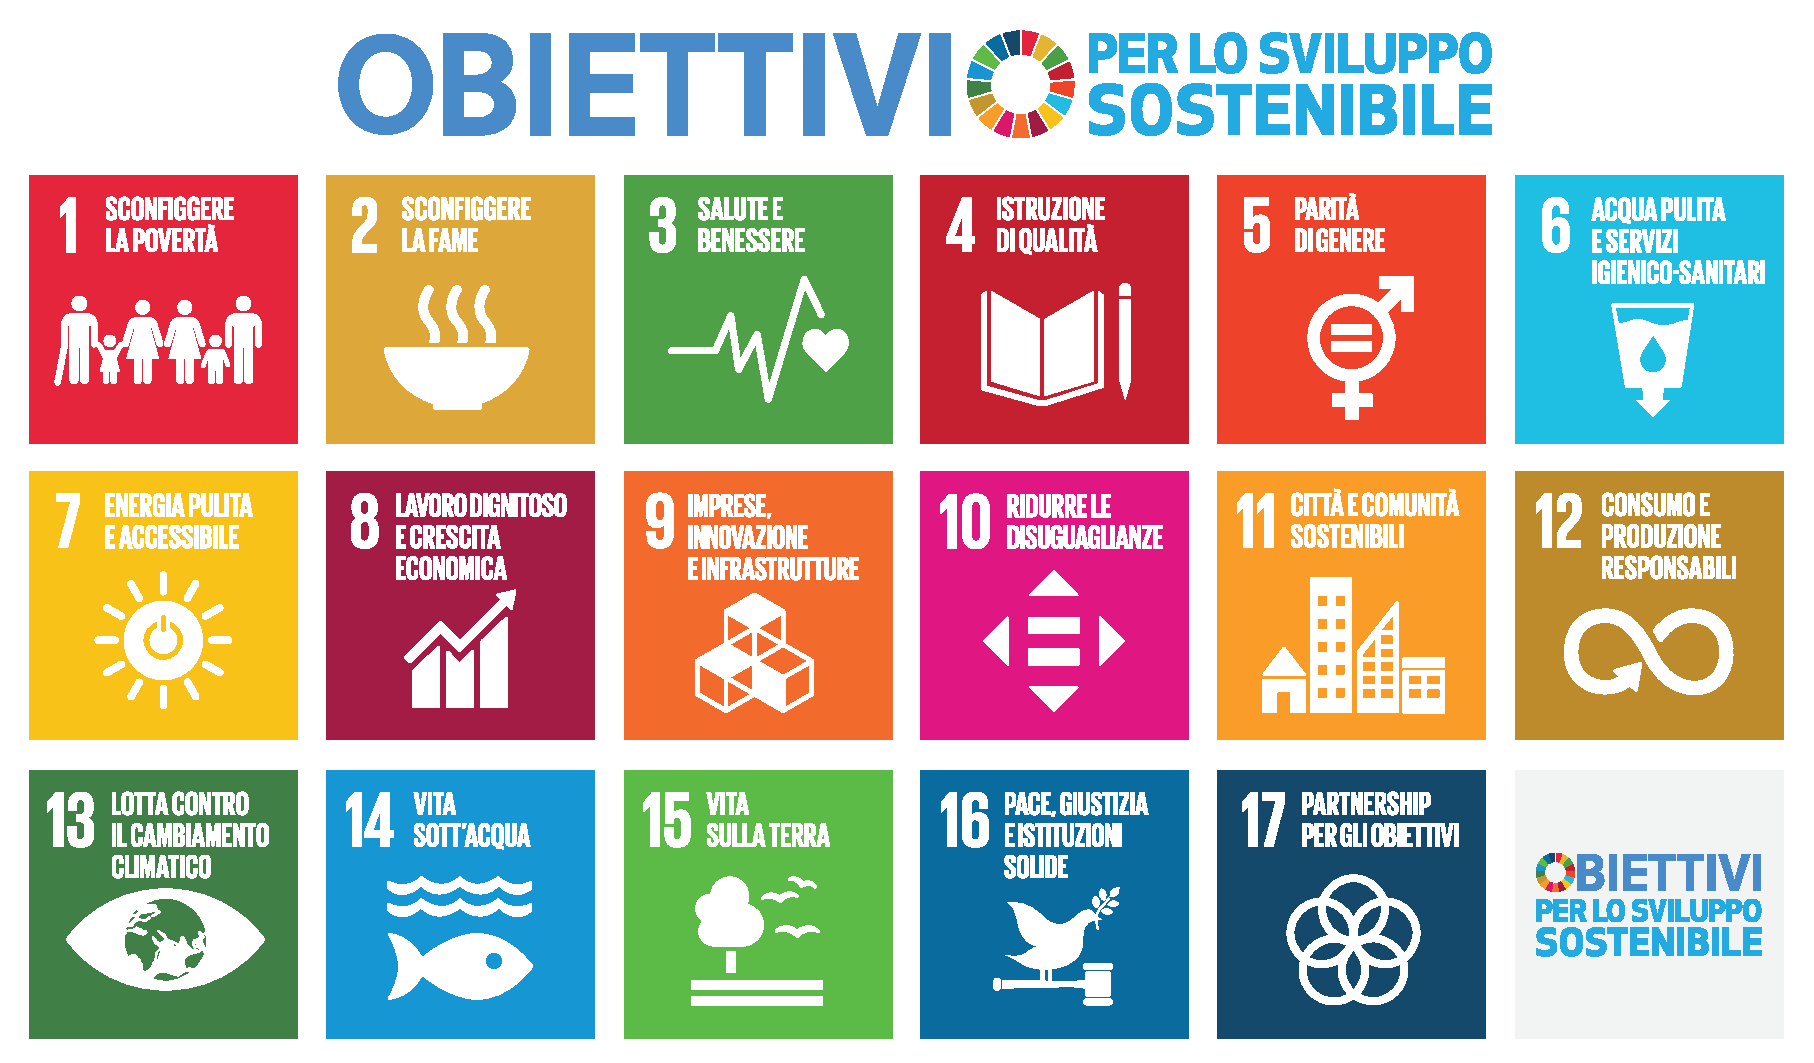
\includegraphics[width=\textwidth]{img/SDG_Poster.png}
    \caption{Grafiche dei 17 Obiettivi per lo sviluppo Sostenibile}
    \label{fig:sdgs}
\end{figure}

\section{Progetto ReMade}

Il progetto ReMade (REplanting for Monitoring Accomplishment of DEmaterialization, \cite{remade_project}), nato con la collaborazione del CESIA, DICAM e DISI Sustainable ICT LAb, fa parte di una serie d'iniziative intraprese dalla Università di Bologna per contribuire al raggiungimento degli Obiettivi per lo Sviluppo Sostenibile.

Lo scopo di questo progetto è quello di potenziare l'effetto del processo di dematerializzazione (riduzione di uso di carta nei processi amministrativi e di comunicazione), traducendo il risparmio di carta nella piantumazione proporzionale di alberi negli spazi verdi e affiancare una \textit{web app} \cite{remadeApp} per diffondere i risultati virtuali (meno carta) e reali (più alberi) al fine di aumentare la consapevolezza da parte della comunità UniBo.

In  questo contesto il contributo di questa tesi mira ad aumentare l'interesse e la consapevolezza sul tema della ecosostenibilità e sul risparmio di carta attraverso l'integrazione di una applicazione per smartphone e un totem multimediale con anche l'aiuto della realtà aumentata e la \textit{gamification}.
\begin{figure}
    \center
    \includegraphics[height=6cm]{img/remade_logo.png}
    \caption{Logo del progetto ReMade}
    \label{fig:remade_logo}
\end{figure}

Con questo progetto l'Ateneo contribuisce a tre degli obiettivi per lo sviluppo sostenibile (Figura \ref{fig:remade_dgs}) che riguardano le città e comunità sostenibili (Goal 11), la lotta contro il cambiamento climatico (Goal 13) e la vita sulla terra (Goal 15); infatti la piantumazione di nuovi alberi porta inevitabilmente a diversi benefici come la riduzione della temperatura, rimozione d'inquinanti atmosferici e miglioramento dello stile di vita e vivibilità delle città.
\begin{figure}
    \centering
    
\includegraphics[width=\textwidth]{img/sdg_remade.png}
    \caption{Obiettivi Agenda 2030 sostenuti dal progetto ReMade}
    \label{fig:remade_dgs}
\end{figure}
\newpage
\section{Motivare gli utenti}
Considerati gli obiettivi del progetto ReMade, al fine di coinvolgere il più possibile la comunità universitaria UniBo, vengono impiegate diverse tecniche come la \textit{Gamification} e l'uso di \textit{Serious games}.
%
%
\subsection{Gamification}
\label{sec:gamification}
Prima di discutere il significato e le implicazioni che il fenomeno della \textit{gamification} sottintende occorre fare una precisazione sui sostantivi inglesi \textit{play} e \textit{game} in quanto assumono sfumature di significato diverso nonostante la loro traduzione in italiano coincida con la parola \enquote{gioco}. Di seguito le definizioni fornite dal \textit{Cambridge Dictionary} \cite{cambridgeDict}:

\begin{description}
    \itemsep1em
    \item [\textit{Play}] \textit{ \enquote*{recreation, amusement}}; attività puramente ricreativa senza regole e obiettivi (es. giocare con giocattoli).
    \item [\textit{Game}] \textit{\enquote*{an activity or sport that people play, usually with rules and needing skill}}; un'attività o sport, dove tipicamente sono presenti regole e sono richieste abilità, il cui scopo è raggiungere uno o più obiettivi (es. giochi da tavolo).
\end{description}

Il termine \textit{gamification} è un termine ombrello informale che indica l'utilizzo di alcuni elementi di gioco (\textit{game elements}) in contesti di tutt'altra natura per migliorare l'esperienza utente (\textit{User Experience UX}) e il suo coinvolgimento \textit{(User Engagement)} \cite{gamificCHI11}.
Al momento non esiste una definizione univoca ma in letteratura ci si riferisce spesso alla strategia della gamification con il concetto di \textit{gameful design} che sottolinea lo scopo di progettare un sistema che sia \textit{gamefulness}, quindi ricco di esperienze e qualità riconducibili al \textit{game} grazie ai suoi elementi e meccanismi \cite{definingGamification2011}.

L'utilizzo della gamification ha avuto un grande successo tanto da esserne immersi nella vita di tutti i giorni. Molti negozi o siti (es. Booking, Figura \ref{fig:booking-genius}) a oggi prevedono un programma fedeltà che comprende l'accumulo di punti per ottenere sconti, molte applicazioni e dispositivi fitness (es. Apple Watch \cite{appleWatchGamification}) sfruttano badge (Figura \ref{fig:appleFitnessBadges}), livelli e sfide periodiche per motivare l'utente a fare movimento (\textit{Games for Health})\cite{game4health}, nel marketing o nelle campagne di crowdfunding (es. KickStarter) la raccolta fondi assume l'aspetto di un gioco con obiettivi e premi e nelle app di navigazione come in Waze ritroviamo un meccanismo di classifica fra gli utenti che possono accumulare punti guidando (Figura \ref{fig:waze-level}).

Questo successo è da ricondursi sicuramente alla natura dell'essere umano che ha un costante desiderio di superare sfide, risolvere problemi e ottenere risultati, tutte esperienze che si ritrovano nei giochi, ma anche alle motivazioni che portano l'utente a giocare (motivazione estrinseca e intrinseca \cite{Deci1975IntrinsicMA}), come ad esempio la soddisfazione o la competizione.

I \textit{game elements}, se utilizzati correttamente, non fanno altro che fare leva sugli aspetti sopra elencati, ottenendo un forte coinvolgimento e divertimento dell'utente che si sentirà anche più motivato.
La definizione di questi elementi non è univoca e di seguito ne vengono presentate due:

\begin{itemize}
    \itemsep1em
    \item la prima è proposta in \citetitle{definingGamification2011}\cite{definingGamification2011} dove vengono identificati cinque elementi su diversi livelli di astrazione:
    \begin{itemize}
        \item \emph{Interface design patterns}: elementi come badge, livelli o classifiche;
        \item \emph{Game design patterns}: per esempio tempo e/o risorse limitate, turni;
        \item \emph{Design principles or heuristics}: gioco duraturo, obiettivi chiari, varietà di stili di gioco;
        \item \emph{Conceptual models of game design units}: modelli concettuali dei componenti o dell'esperienza di gioco;
        \item \emph{Game design methods}: pratiche e processi specifici per la progettazione del gioco.
    \end{itemize}
    %
    \item la seconda invece in \citetitle{Werbach2012ForTW}\cite{Werbach2012ForTW} che vede tre elementi chiave:
    \begin{itemize}
        \item \emph{Components}: tra cui punti, badge, livelli, missioni, classifiche, regali da condividere;
        \item \emph{Mechanics}: comprende i processi che guidano l'azione in avanti e generano coinvolgimento nel giocatore, ad esempio la cooperazione o competizione con altri utenti, turni di gioco, stati di vittoria, ricompense
        \item \emph{Dynamics}: aspetti da considerare e gestire come narrativa, crescita e sviluppo del giocatore, interazioni sociali, emozioni provate durante il gioco
    \end{itemize}
\end{itemize}


\begin{figure}
    \centering
    \subfloat[App Fitness di Apple: schermata con premi e obiettivi]{
        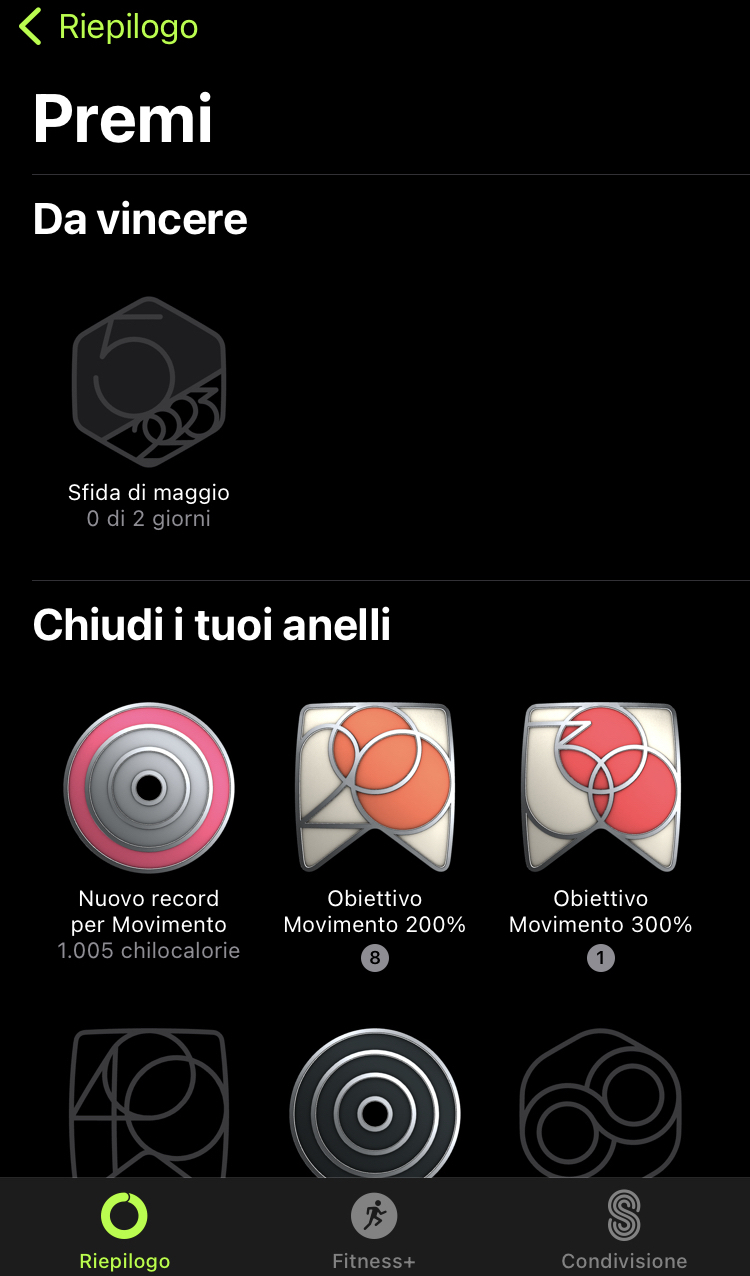
\includegraphics[width=0.4\textwidth]{img/apple-fitness-badge.jpeg}
        \label{fig:appleFitnessBadges}
    }
    \hspace{2em}% Space between image A and B
    \subfloat[Programma fedeltà Genius di Booking: sconti in base al livello]{
        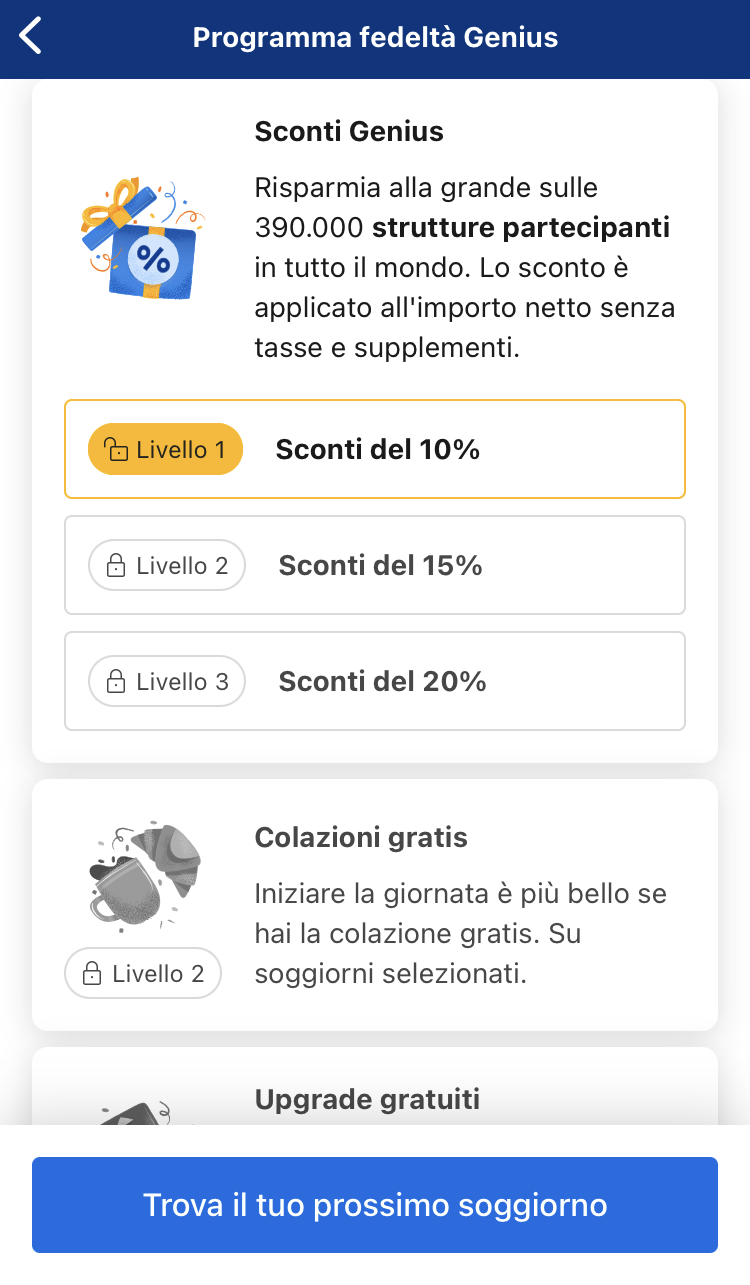
\includegraphics[width=0.4\textwidth]{img/booking-gamification.PNG}
        \label{fig:booking-genius}
    }
    \hspace{2em}% Space between image B and C
    \subfloat[App navigatore stradale Waze: tabellone punti e livello utente]{
        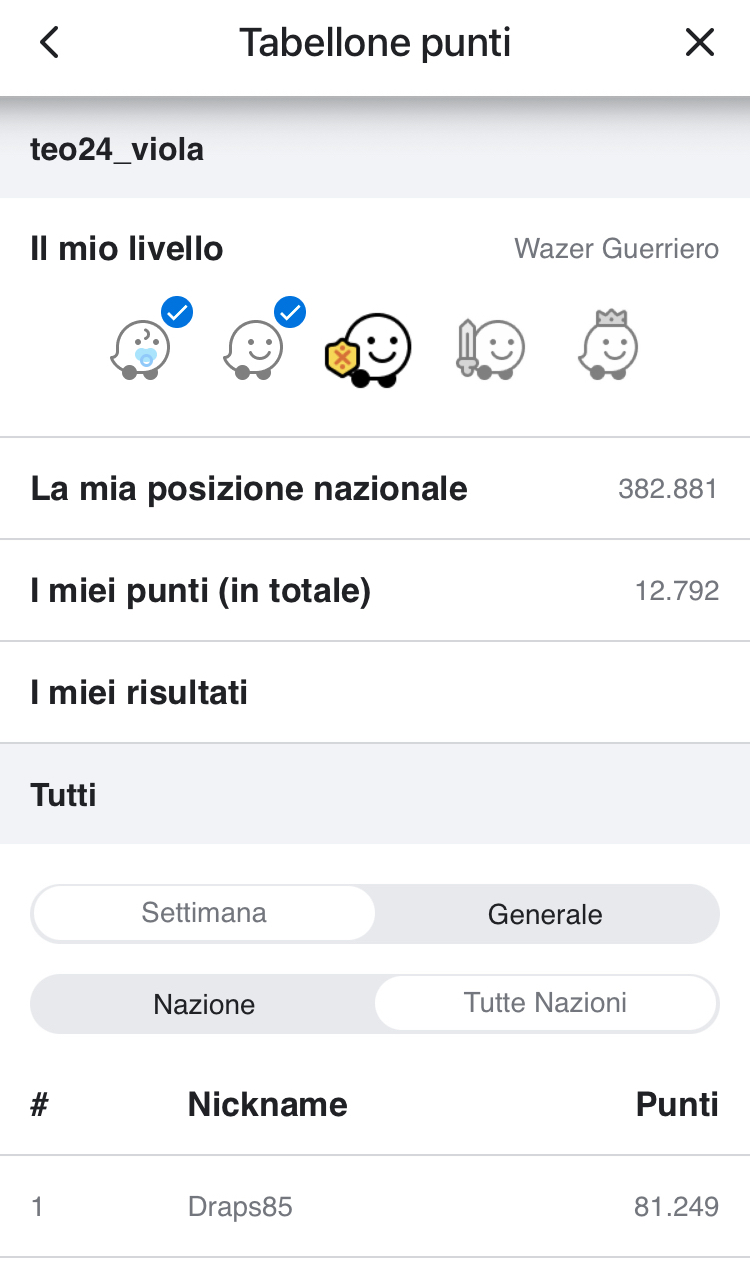
\includegraphics[width=0.4\textwidth]{img/waze2.jpeg}
        \label{fig:waze-level}
    }
    \caption{Esempi di piattaforme e app dove è presente la \textit{gamification}} 
    \label{fig:gamification-example}
\end{figure}
%
%
\subsection{Serious game}
I \textit{Serious games} sono giochi sviluppati con il principale intento di educare, formare e in secondo luogo intrattenere, in modo da rendere più piacevole, interessante ed efficace l'apprendimento; nel caso vengano utilizzati supporti tecnologici si parla di \textit{Plugged Gamification}(es. Kahoot, Duolingo, AR, VR, \dots), altrimenti di \textit{Unplugged Gamification} (es. Quiz, puzzle, gare di teoria a squadre, \dots) \cite{pluggedGamificSeriousGame}.

I \textit{serious game} presentano degli obiettivi chiari e precisi che verranno raggiunti dopo che l'utente avrà imparato qualcosa di nuovo.


\textcolor{red} {todo: parlare di esempi di serious game e del loro effetto positivo sull'apprendimento \cite{seriousgame_langLearn}}


% Alcune delle cose che i giochi fanno bene includono incoraggiare la risoluzione dei problemi, sostenere l'interesse da principiante a esperto da padroneggiare, scomporre le grandi sfide in passi gestibili, promuovere il lavoro di squadra, dare ai giocatori un senso di controllo, personalizzare l'esperienza per ogni partecipante, premiare il pensiero fuori dagli schemi, ridurre la paura del fallimento che inibisce la sperimentazione innovativa, sostenere

% È stato dimostrato che questo genere di giochi possono migliorare l'attenzione e l'apprendimento se progettati correttamente;
% sono presenti studi che dimostrano che l'utilizzo di Serious Game aumenta l'efficacia dell'apprendimento da parte di studenti, e in alcuni casi anche grazie all'aiuto di tecnologie come la Realtà Estesa, Aumentata e Virtuale.
% Si cita uno dei tanti studi condotti per verificare l'efficacia di utilizzare la Realtà Estesa (AR, VR, MR) per insegnare in ambito medico ed effettuare simulazioni di operazioni chirurgiche dove è risultato che solo il 7\% dei casi non c'è stata maggiore efficacia nell'apprendimento \cite{HMDmedicalSeriousgame}, mentre nel resto degli altri casi c'è stata maggior motivazione, coinvolgimento ed efficacia da parte degli studenti.

%
\section{Extended Reality}
Extended Reality (XR), in italiano Realtà Estesa, è un termine che raggruppa tutte le possibili realtà che si possono generare utilizzando sistemi elettronici e informatici per portare una o più persone in realtà potenziate o totalmente generate dal computer.
Si identificano tre tipologie:

\begin{itemize}
    \item \textbf{Realtà Aumentata (AR)}: l'ambiente reale circostante viene integrato con oggetti virtuali e/o informazioni utili aggiunti digitalmente;
    \item \textbf{Realtà Virtuale (VR)}: la realtà circostante viene completamente sostituita con una virtuale;
    \item \textbf{Realtà Mista (MR)}: il mondo reale e la realtà virtuale coesistono in una unica realtà
\end{itemize}

Per poter di utilizzare e sfruttare le potenzialità di queste realtà, sono disponibili svariate tecnologie hardware. Di seguito un elenco, sicuramente non esaustivo, dei principali dispositivi presenti sul mercato:

\begin{itemize}
    \item \textit{Head-Mounted Devices} (HMDs), grazie ai sensori e alle videocamere presenti, le interazioni possono avvenire usando il movimento della testa (\textit{Hand-free}), con controller oppure  attraverso le proprie mani senza la necessita di ulteriori dispositivi, 
    \item Smartphone e tablet, attraverso lo schermo e grazie alla videocamera e i sensori è possibile utilizzare l'AR
    \item Smart Glasses, occhiali per l'AR
    \item Tute e guanti aptici, per la realtà virtuale, che permettono di trasmettere sensazioni tattili, tracciare il movimento del corpo e i dati biometrici e gestire la temperatura rendendo l'esperienza virtuale il più reale possibile;
    \item Tapis roulant per simulare il movimento nel mondo in VR
\end{itemize}

\subsection{Realtà aumentata}
\label{sec:ar}
La Realtà Aumentata (in inglese Augmented Reality, AR) consiste nell'arricchire il mondo reale circostante con oggetti e informazioni multimediali di vario genere e tipologia che normalmente non sarebbero percepibili dai cinque sensi. % Per alcuni si tratta di semplici sovrapposizioni d'informazioni attinenti al contesto in cui l'utente si trova mentre per altri affinché sia AR è necessaria una registrazione spaziale e/o una interazione con lo spazio circostante. \cite[ Capitolo 4, What is AR?]{whatMR}
Questi arricchimenti sono fruibili per mezzo di dispositivi come ad esempio visori AR, computer provvisti di webcam, smartphone, auricolari, lenti a contatto o tecniche particolari come il Video Mapping che fa uso di proiezioni sulle superfici e oggetti senza la necessità d'indossare alcun dispositivo (Spatially Argumented Reality\cite{Raskar1999SpatiallyAR}).

Si identificano tre tipologie di AR che si differenziano in base al criterio utilizzato per il posizionamento degli elementi \enquote{aumentanti} nell'ambiente circostante; si hanno quindi Realtà Aumentate:

\begin{description}
    \item \textbf{\textit{Location-based}} (Figura \ref{fig:location_ar}) dove gli elementi vengono disposti in una precisa posizione geografica GPS, ad esempio viene mostrata una icona in corrispondenza di punti d'interesse (POI) in tempo reale, o viene emesso un suono specifico in corrispondenza di uno di questi;
    \item \textbf{\textit{Marker-based}} (Figura \ref{fig:marker_ar}), gli oggetti vengono sovrapposti e posizionati sul marker che può essere un codice QR, una immagine o un disegno;
    \item \textbf{\textit{Markerless}} (Figura \ref{fig:markerless_ar}), dopo una scansione dell'ambiente circostante, ad esempio con la fotocamera dello smartphone, gli oggetti vengono collocati su quelle caratteristiche ambientali ritenute adatte (es. superfici orizzontali o verticali).
\end{description}

\begin{figure}
    \centering
    \subfloat[Funzionalità Live View in Google Maps che utilizza l'AR Location-based]{
        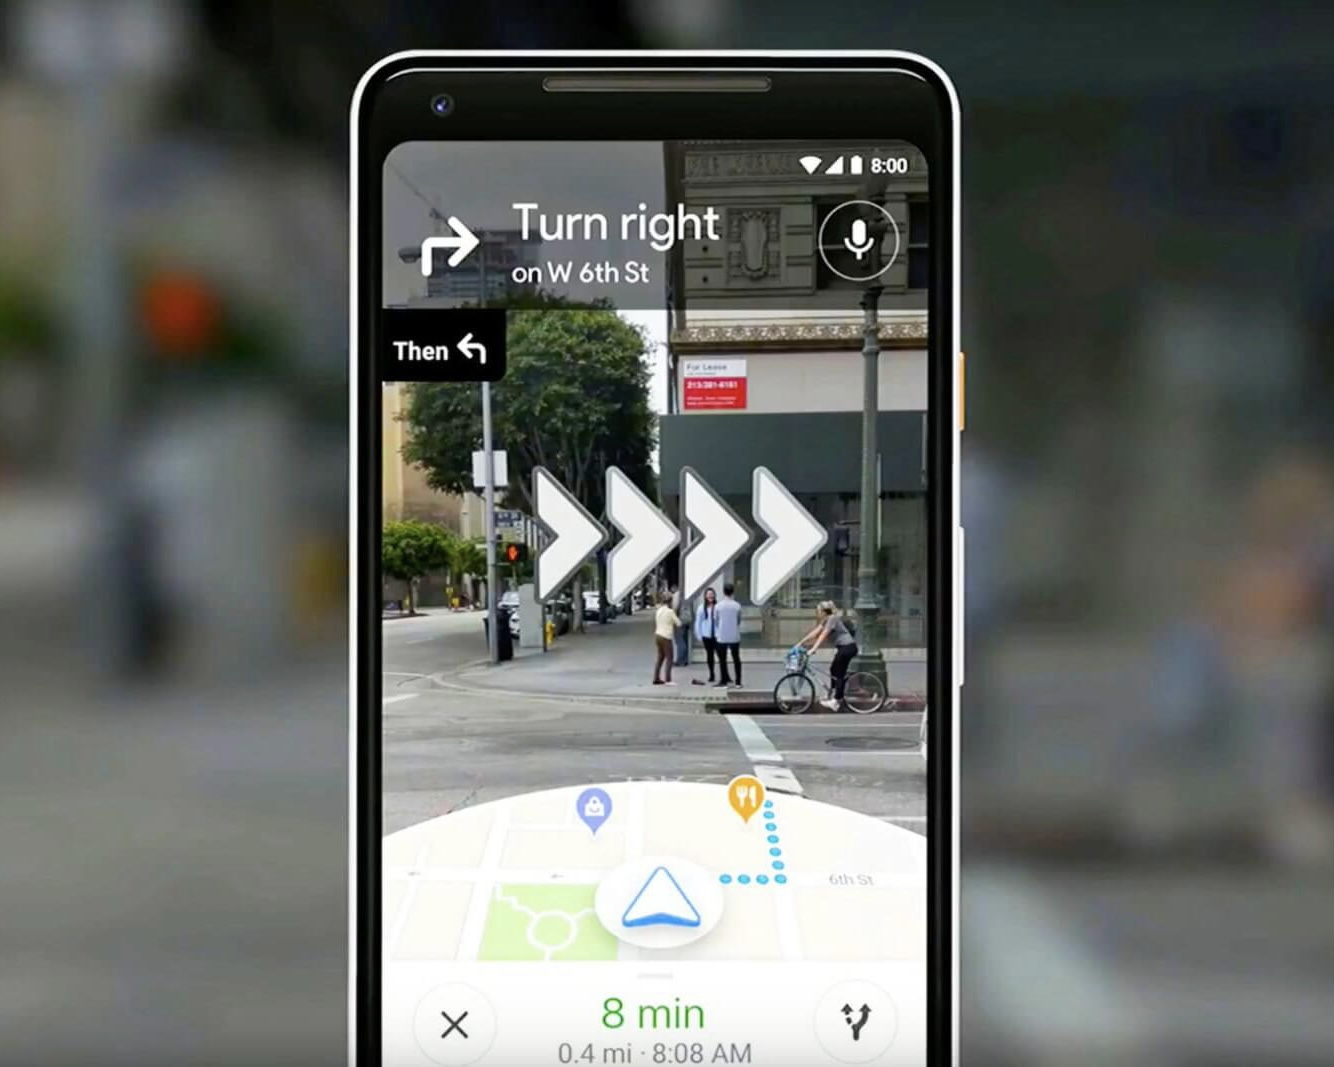
\includegraphics[width=0.32\textwidth]{img/location-based-ar.jpg}
        \label{fig:location_ar}
    }
    \subfloat[Marker-based AR]{
        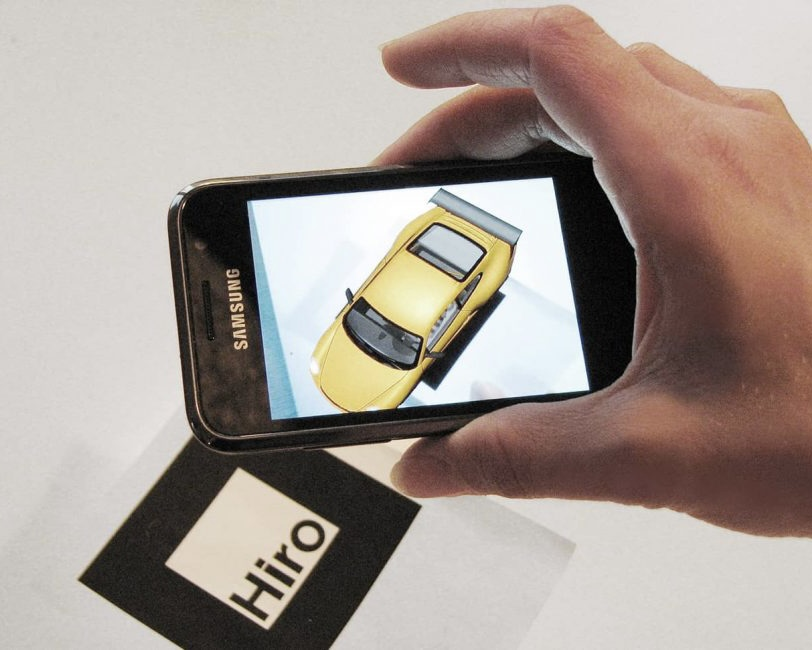
\includegraphics[width=0.32\textwidth]{img/marker-base-ar.jpg}
        \label{fig:marker_ar}
    }
    \subfloat[Markerless AR: App IKEA Place]{
        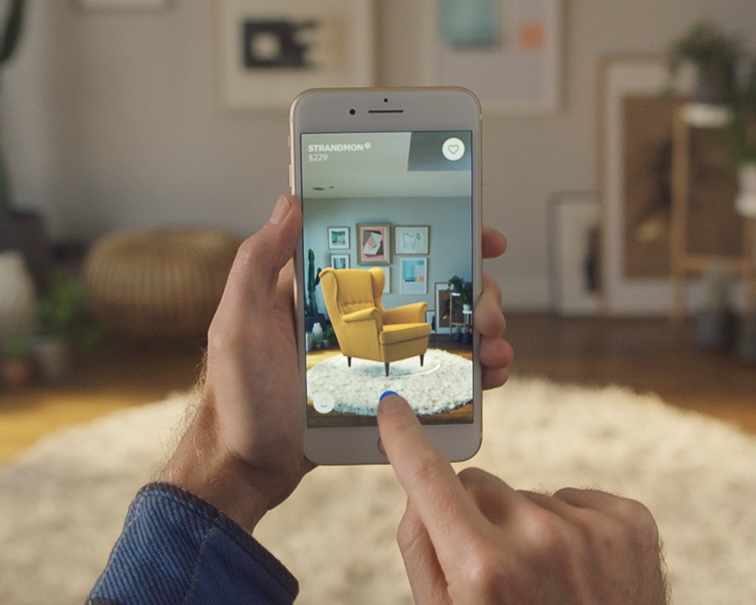
\includegraphics[width=0.32\textwidth]{img/markerless-ar.jpg}
        \label{fig:markerless_ar}
    }
    \caption{Esempi di tre tipologie di Realtà Aumentata} 
    \label{fig:ARbased_type}
\end{figure}

Nel settore educativo l'utilizzo di questa tipologia di tecnologia ha permesso d'integrare, e insegnare interamente in alcuni casi, con contenuti virtualmente aggiunti come potrebbe essere un dinosauro sulla cattedra o \dots TODO

\subsection{Realtà Virtuale}
La Realtà Virtuale (in inglese Virtual Reality, VR) sostituisce l'ambiente circostante con uno che realmente esiste (es. simulazioni) o completamente virtuale (es. videogiochi), isolando l'utente da tutte le interazioni sociali esterne. Questo genere di realtà sono necessari dispositivi hardware indossabili specifici come gli head mounted displays (HMD)\dots

\subsection{Mixed reality}

%
\section{Integrazione tra diversi tipi di device}
\section{Integrazione tra totem e smartphone}